\chapter{Background}
\label{Chapter2}

This chapter provides important background information about cube that
will facilitate understanding the topics presented in later chapters.
Section \ref{sec:rubiks-history} will describe the historical origin of
the cube. Then, Section \ref{sec:rubiks-anatomy} will detail the
structure of the cube and the notation used to transcribe move
sequences. Finally, Section \ref{sec:speedsolving} will outline the
culture and regulations surrounding competitive speedsolving.


\section{A Brief History of the Rubik's Cube}
\label{sec:rubiks-history}

In 1974, Erno Rubik, a Hungarian professor of architecture, sought to
help his students visualize space in three dimensions. To that end, he
created a special cube whose faces could independently rotate around
all three physical axes \cite{rubik-motivation}. When he added colored
stickers to further aid in visualizing the movements, Mr. Rubik
realized he had created a new puzzle. He patented his cube in 1975,
\cite{rubik-patent} and since then over 450 million units have been
sold \cite{forbes-rubik-merger}, allowing an estimated 1 in 7 humans on
earth to try their hand at solving it \cite{rubik-population-reached}.


\section{The Anatomy of a Rubik's Cube}
\label{sec:rubiks-anatomy}

The Rubik's Cube, like a standard geometric cube, has six square faces
positioned at right angles to each other. When solved, each of these
faces has a single, unique color.

The Rubik's Cube is further subdivided into a 3x3x3 arrangement of
smaller "cubies" such that each face consists of nine individual
colored stickers/tiles (see Figure \ref{fig:anatomy-cube}). There are
three different types of cubies - centers, edges, and corners - each
which is distinguished by the number of unique colors it binds together
into a single physical unit. The six center cubies have one color each
(see Figure \ref{fig:anatomy-centers}), the twelve edges have two
colors each (see Figure \ref{fig:anatomy-edges}), and the eight corners
have three colors each (see Figure \ref{fig:anatomy-corners}).

Each of the six center cubies are also attached to a common core which
allows them to rotate freely, but fixes their position relative to each
other. As such, the single color of each center cubie is also the color
shared by the corresponding face when the entire cube is solved.

\newpage
\null  % Vertical centering: https://www.reddit.com/r/LaTeX/comments/1crepl/center_figure_vertically_on_new_page/
\vfill
% How to do a sub-figure: https://tex.stackexchange.com/a/37597
\begin{figure}[h]
    \centering
    \caption{The Anatomy of the Rubik's Cube \cite{iamthecube}}
    \label{fig:anatomy}
    \begin{subfigure}{0.5\textwidth}
        \centering
        \caption{Full Cube}
        \label{fig:anatomy-cube}
        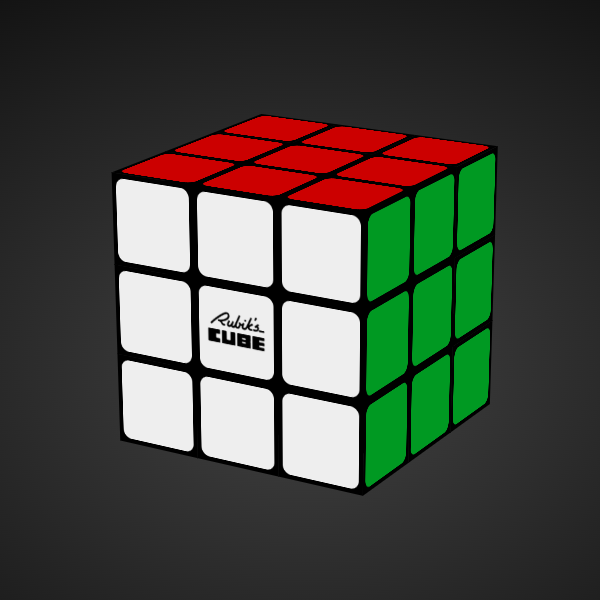
\includegraphics[width=.90\linewidth]{Figures/2 Background/anatomy-cube.png}
    \end{subfigure}%
    \begin{subfigure}{0.5\textwidth}
        \centering
        \caption{Centerpieces}
        \label{fig:anatomy-centers}
        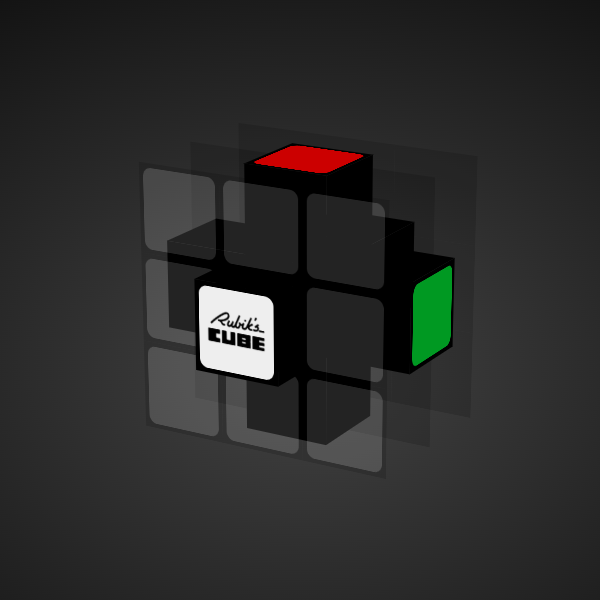
\includegraphics[width=.90\linewidth]{Figures/2 Background/anatomy-centers.png}
    \end{subfigure}\\
    \vspace{2mm}
    \begin{subfigure}{0.5\textwidth}
        \centering
        \caption{Edges}
        \label{fig:anatomy-edges}
        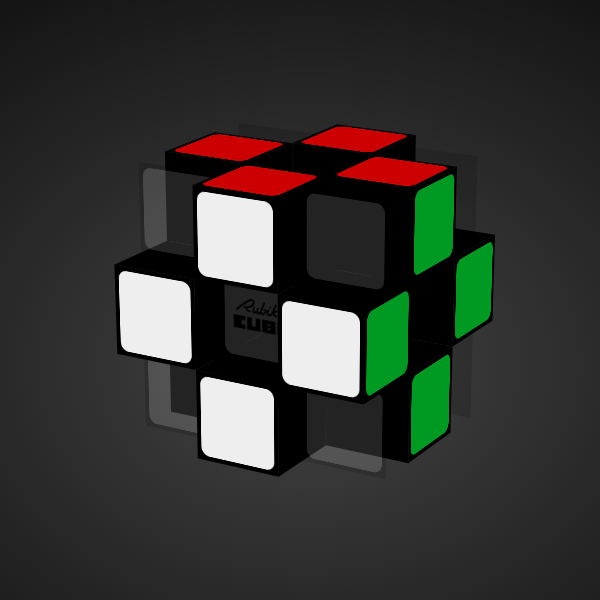
\includegraphics[width=.90\linewidth]{Figures/2 Background/anatomy-edges.png}
    \end{subfigure}%
    \begin{subfigure}{0.5\textwidth}
        \centering
        \caption{Corners}
        \label{fig:anatomy-corners}
        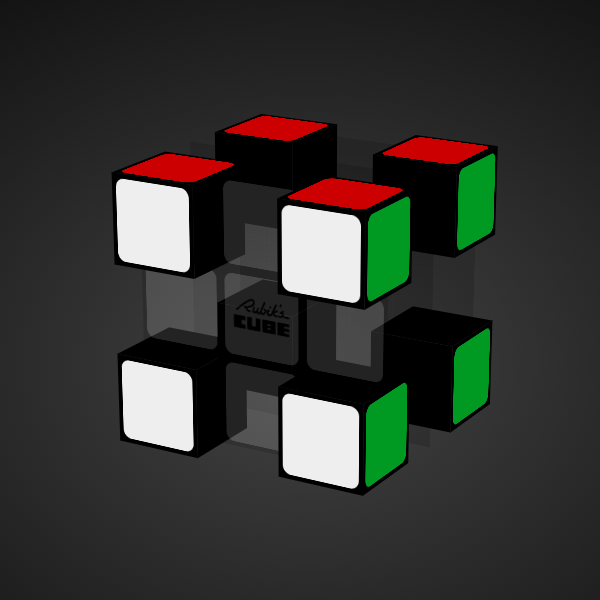
\includegraphics[width=.90\linewidth]{Figures/2 Background/anatomy-corners.png}
    \end{subfigure}\\
\end{figure}
\vfill
\newpage

\subsection{Move Sequence Notation}
\label{subsec:algorithm-notation}

Shortly after the cube's invention, David Singmaster, a British
mathematician, proposed a beginner-friendly, layer-by-layer approach to
solving the cube. To facilitate communication of his solution, he
outlined a notation for documenting the face turns required for each
phase. This notation, now known as the Singmaster Notation, has become
the standard notation used for documenting move sequences for the cube.
\cite{singmaster-notation}

The notation consists of two components: (1) A label for each face of the
cube and (2) a superscript to indicate a direction of rotation.

The labels for each face are as follows:

\begin{itemize}
    \item $U$ - "Up": The top face
    \item $D$ - "Down": The bottom face
    \item $R$ - "Right": The "Right" side face
    \item $L$ - "Left": The "Left" side face
    \item $F$ - "Front": The face directly in "Front" of the solver
    \item $B$ - "Back": The face on the "Back" side of the cube facing away from the solver
\end{itemize}

Notice that the labels for each face are assigned based on its relative
orientation, not the color of its centerpiece. For example, the top
face is always labelled $U$ whether the top facing centerpiece is
green, yellow, or another color. This is demonstrated by the
color-neutral image used to depict these face labels in Figure
\ref{fig:cube-notation}.

\begin{figure}[h]
    \centering
    \caption[Rubik's Cube Notation]{Notational names for each face of the Rubik's Cube \cite{img-cube-notation}}
    \label{fig:cube-notation}
    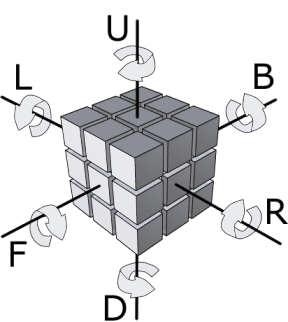
\includegraphics{Figures/2 Background/rubik's_cube_notation_bw.png}
\end{figure}

\newpage
The superscripts are as follows:

\begin{itemize}
    \item $X^1$ : 90$^o$ Clockwise rotation. Generally abbreviated as \code{X}
    \item $X^{-1}$ : 90$^o$ Counter-clockwise rotation. Generally abbreviated as \code{X'}
    \item $X^2$ : 180$^o$ Rotation. Generally abbreviated as \code{X2}
\end{itemize}

For example, the move sequence \code{R U2 R'} denotes turning the Right
layer 90$^o$ clockwise, followed by a 180$^o$ rotation of the Up face,
and finalized by a 90$^o$ counter-clockwise rotation of the Right face
(see Figure \ref{fig:notation-demo})\footnote{Images generated with the
Twizzle Editor found at
\href{https://alpha.twizzle.net/edit/?alg=R+U2+R\%27}{alpha.twizzle.net}}.

% How to do a sub-figure: https://tex.stackexchange.com/a/37597
\begin{figure}[h]
    \centering
    \caption{The move sequence \code{R U2 R'}}
    \label{fig:notation-demo}
    \begin{subfigure}{0.25\textwidth}
        \centering
        \caption{Starting Cube}
        \label{fig:notation-demo-start}
        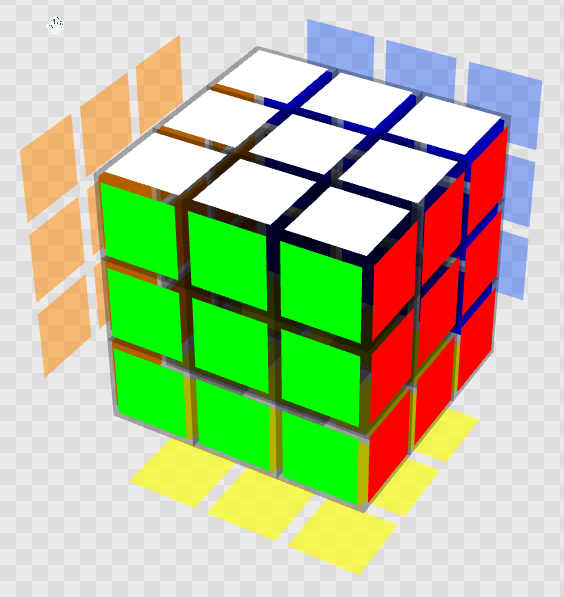
\includegraphics[width=.90\linewidth]{Figures/2 Background/start.png}
    \end{subfigure}%
    \begin{subfigure}{0.25\textwidth}
        \centering
        \caption{Apply \code{R}}
        \label{fig:notation-demo-r}
        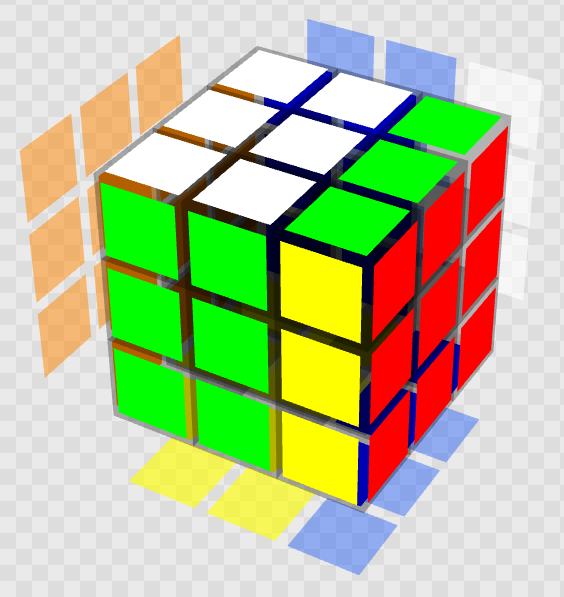
\includegraphics[width=.90\linewidth]{Figures/2 Background/R.png}
    \end{subfigure}%
    \begin{subfigure}{0.25\textwidth}
        \centering
        \caption{Apply \code{U2}}
        \label{fig:notation-demo-u2}
        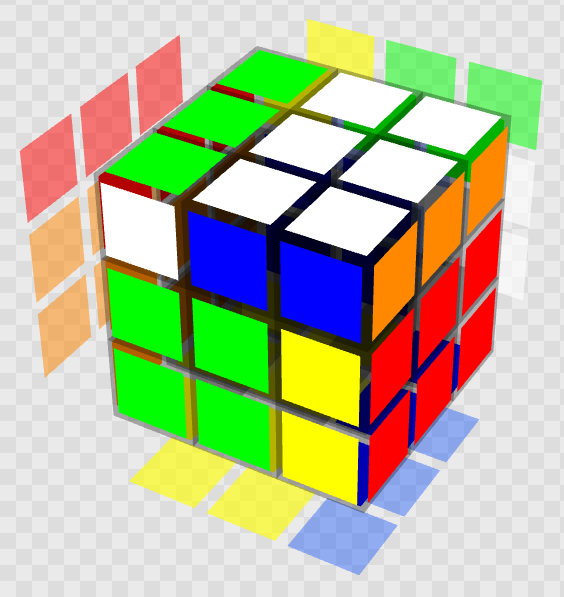
\includegraphics[width=.90\linewidth]{Figures/2 Background/U2.png}
    \end{subfigure}%
    \begin{subfigure}{0.25\textwidth}
        \centering
        \caption{Apply \code{R'}}
        \label{fig:notation-demo-rprime}
        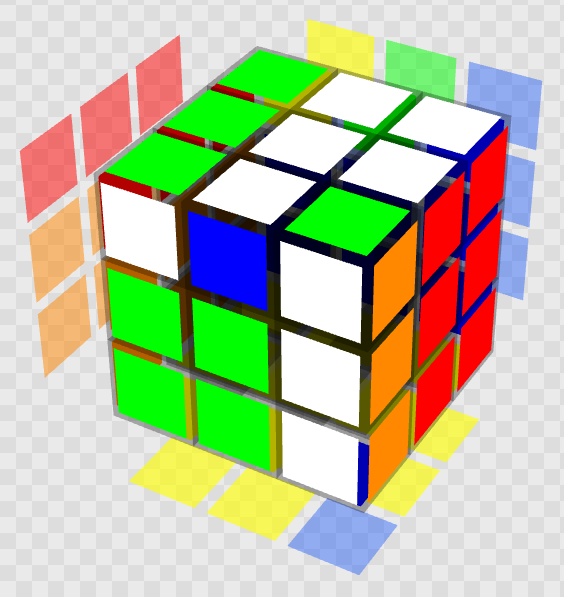
\includegraphics[width=.90\linewidth]{Figures/2 Background/R'.png}
    \end{subfigure}%
\end{figure}


\section{A Brief History of Speedsolving}
\label{sec:speedsolving}

As more people learned to solve the cube, there began to be increased
interest in solving the cube as quickly as possible. In 1982, the first
Rubik's Cube World Championship was held in Budapest with a winning
solution time of 22.95 seconds by Minh Thai. However, due to falling
interest, no further competitions were organized in the following two
decades.

Interest in speedcubing picked back up in the late 1990s as the
consumer internet facilitated sharing of strategies and techniques. In
2003, the second competition, the World Rubik's Games Championship
2003, was held in Toronto, Canada with 89 competitors and a winning
average time of 20.00 seconds. Additional competitions were organized
later that year and into 2004. \cite{wca-speedcubing-history}

\subsection{The World Cube Association}
\label{subsec:the-world-cube-association}

To provide a set of standard regulations for the increasing number of
speedcubing competitions, the World Cube Association (WCA) was founded
in August 2004 by Tyson Mao and Ron van Bruchem. Today, the WCA governs
all official speedcubing competitions by creating and enforcing a
consistent set of regulations, providing tools for creating fair
scrambles, and hosting the official platform for sharing competitions
results. \cite{wca-speedcubing-history}

\subsection{The Rise of Smartcubes}
\label{subsec:the-rise-of-smart-cubes}

In September 2018, the Xiaomi released the Giiker Cube, the first cube
with built-in sensors to track its face turns during use.
\cite{giiker-thecubicle} For the first time, a solution could be
analyzed without first requiring the tedious process of transcribing
each individual move from a video recording! Additional "smartcubes"
were released by a variety of manufacturers in the following years.
\cite{gocube-product-launch-video} \cite{gans356i-thecubicle}
\cite{gocube-rubiksconnected}

However, despite their usefulness during personal practice, smartcubes
cannot be used in official competitions. According to WCA regulation
2i, "While competing, competitors must not use electronics or audio
equipment (e.g. cell phones, MP3 players, dictaphones, additional
lighting) apart from the Stackmat timer or stopwatch."
\cite{wca-regulations} This protects against competitors gaining unfair
inspection time by previewing the scrambled cube from a connected
device before it is brought to the competition table.
